%%% Research Diary - Entry
%%% Modified from Mikhail Klassen, April 2013
%%% 
\documentclass[10pt,letterpaper]{article}

% To add your univeristy logo to the upper right, simply
% upload a file named "logo.png" using the files menu above.
\usepackage[colorlinks=true,citecolor=blue,linkcolor=blue]{hyperref}
\usepackage{graphicx}
\usepackage{epstopdf}
\usepackage{epsfig} %% for loading postscript figures
\usepackage{subfigure} 
\usepackage{amsmath}
\usepackage{tikz}
\usepackage[margin=1.25in]{geometry}

\newcommand*\circled[1]{\tikz[baseline=(char.base)]{\node[shape=circle,draw,inner sep=1pt] (char) {#1};}}



\begin{document}
\section{Wavy Interface}
\subsection{Previous work}
Wavy interfaces are a prominent architectural motif in architectured SBs, such as woodpecker beaks (see Figure~\ref{fig:VRF-WI}~(b)) and the cranial bones of rams, that are subjected to impact or cyclic loads but must remain intact to perform their mechanical functions \cite{lee2014hierarchical, jaslow1990mechanical}.


% In experiments that involve contact with adhesion between two surfaces, as found in atomic force microscopy (AFM) or nano-indentation, two distinct contact force ($P$) versus indentation depth ($h$) curves are often found depending on whether the indenter moves towards or away from the sample (see Figure~\ref{fig:DDHAFM} (a)). 
% %
% Specifically, the surfaces appear more adhesive during the unloading stage and less adhesive during the loading stage. This phenomenon is termed adhesion hysteresis and has been observed in a wide variety of experiments involving compliant (e.g. elastomeric) surfaces [REF]. 
% %
% The hysteretic energy loss is observed to depend on the maximum indentation depth (marked $|h_{\rm min}|$ in Figure~\ref{fig:DDHAFM} (a)) in a load-unload cycle.
% %
% The classical adhesive, elastic contact theories [REF] do display hysteresis, however the hysteresis captured by them is qualitatively different from the one observed in experiments and the predicted energy loss is independent of $|h_{\rm min}|$.
% %
% The origin of the hysteresis in experiments was not well understood and is often attributed to moisture, plasticity, viscoelasticity, or material-specific mechanisms such as polymer interdigitation [REF].

In experiments that involve contact with adhesion between two surfaces, two distinct contact force ($P$) versus indentation depth ($h$) curves are often found depending on whether the indenter moves towards or away from the sample (see Figure~\ref{fig:DDHAFM} (a)). 
%
Moreover, the hysteretic energy loss is observed to depend on the maximum indentation depth (marked $|h_{\rm min}|$ in Figure~\ref{fig:DDHAFM} (a)) in a load-unload cycle.
%
The PI's experiments [REF] and continuum mechanics based theoretical work [REF] showed that the hysteresis can exist without moisture, plasticity, or viscoelasticity and that its magnitude depends on surface roughness. 
%
The continuum mechanics models involved approximating the surface roughness with axisymmetric waviness of wavelength $\lambda$. 
%
As seen in Figure~\ref{fig:DDHAFM} (b), the surface waviness can create many metastable states for the contact interface at each value of the loading parameter $h$. 
%
The hysteresis results from the fact that the system visits the state with the smallest contact size during the loading stage and the state with the largest contact size during the unloading stage (Figure~\ref{fig:DDHAFM} (b)). 
%
The energy loss is the result of a series of surface instabilities (marked with dashed magenta lines in Figure~\ref{fig:DDHAFM} (b)), in which the contact area grows or recedes by a finite amount. 
%
As $|h_{\rm min}|$ increases, so do the number of instabilities and hence the energy loss.
%
Studying the asymptotic behavior of the continuum theory in the limit $\lambda \to 0$(Figure~\ref{fig:DDHAFM} (b)--(c)), it was found that the ($h$, $P$) points measured in an experiment would satisfy the equations
%
\begin{subequations}
\label{eq:P-h}
\begin{align}
	P(a) &= \frac{4E^*}{3R}a^3 - \sqrt{8\pi w E^*} a^{3/2} \pm 2\pi E^* A \lambda^{1/2} a^{3/2}, \label{eq:P}\\
	h(a) &= \frac{1}{R}a^2 - \sqrt{\frac{2\pi w}{E^*}}a^{1/2} \pm \pi A \lambda^{1/2} a^{1/2}, \label{eq:h}
\end{align}
\end{subequations}
%
where $a$ is the contact radius, $E^*$ the plane strain Young's modulus, $A$ is the amplitude of the surface
waviness, and $R$ is the radius of the spherical indenter. 
%
The $+$ and $-$ signs correspond to the loading and unloading stages of the experiment, respectively. 
%
The Eqs.~\eqref{eq:P}--\eqref{eq:h} reveal that even though the intrinsic work of adhesion, $w$, remains constant, the experiments measure a higher effective work of adhesion of $w_{\rm eff}^{1/2} = w^{1/2} + A(\pi E^* \lambda/2)^{1/2}$ during the loading state and a lower value of $w_{\rm eff}^{1/2} = w^{1/2} - A(\pi E^* \lambda/2)^{1/2}$ during the unloading state. 
%
%
\begin{figure}[h]
	\includegraphics[width=\textwidth]{../../Proposal/ProjectDescription/Figures/WavyInterface/DDHAFM.pdf}
	\centering
	\caption{(a) The contact force $P$ as a function of indentation depth $h$ (shown marked in (a)) during contact of glass and PDMS in air at an indenting rate of $\dot{d}$ = 10 nm/s, (b) the $P$--$h$ curves predicted by a smooth-surface contact model and by wavy-surface (``rough'') contact model, and (c) the measured $P$--$h$ curve described by Eqs.~\eqref{eq:P}--\eqref{eq:h} that are derived by studying the asymptotic behavior of wavy-surface contact model in the limit of $\lambda \to 0$ (figure adapted from [REF]).}
	\label{fig:DDHAFM} 
\end{figure}



Therefore, based on his previous studies of adhesion between wavy surfaces, the PI believes that the wavy interfaces could be a key ingredient for enhancing the toughness of these materials \cite{li2012numerical,wang2012specific,zavattieri2007determination,haghpanah2014adhesively}. 
%
Even though the interface's intrinsic adhesion energy is constant, the interface's waviness can increase the measured --- i.e., the effective --- adhesion energy. 
%
Similar adhesion energy enhancement has been reported for thin films with adhesive heterogeneities~\cite{xia2015adhesion}. 
%
Motivated by this discovery and the similarities between the mechanics of contact and fracture, the PI searched for new toughening mechanisms in materials with wavy interfaces.


\subsection{Previous work--Short version}
Wavy interfaces are a prominent architectural motif in architectured SBs, such as woodpecker beaks (see Figure~\ref{fig:VRF-WI}~(b)) and the cranial bones of rams, that are subjected to impact or cyclic loads but must remain intact to perform their mechanical functions \cite{lee2014hierarchical, jaslow1990mechanical}.

Recently, the PI experimentally found that surface roughness can give rise to depth-dependent-hysteresis (DDH) [REF].
%
Moreover, he found that the energy loss due to DDH could increase with the surface roughness, which is equivalent to an adhesive toughening of the contact interface.
%
He further proposed a continuum mechanics based model of adhesive elastic contact between rough surfaces, in which the surface roughness is approximated with axisymmetric waviness of amplitude $A$ and wavelength $\lambda$ [REF]. 
%
The hysteretic energy loss of DDH is emerged as the smeared out effect of a series of small-scale surface waviness created mechanical instabilities that take place at the growing and the receding edges of the contact interface. 
%
Studying the asymptotic behavior of the continuum theory in the limit $\lambda \to 0$, it was found that the contact force $P$ and indentation depth $h$ are
\begin{subequations}
\label{eq:P-h}
\begin{align}
	P(a) &= \frac{4E^*}{3R}a^3 - \sqrt{8\pi w E^*} a^{3/2} \pm 2\pi E^* A \lambda^{1/2} a^{3/2}, \label{eq:P}\\
	h(a) &= \frac{1}{R}a^2 - \sqrt{\frac{2\pi w}{E^*}}a^{1/2} \pm \pi A \lambda^{1/2} a^{1/2}, \label{eq:h}
\end{align}
\end{subequations}
%
where $a$ is the contact radius, $E^*$ is the plane strain Young's modulus, and $R$ is the radius of the spherical indenter. 
%
The $+$ and $-$ signs correspond to the loading and unloading stages of the experiment, respectively. 
%
The Eqs.~\eqref{eq:P}--\eqref{eq:h} reveal that even though the intrinsic work of adhesion, $w$, remains constant, the experiments measure a higher effective work of adhesion of $w_{\rm eff}^{1/2} = w^{1/2} + A(\pi E^* \lambda/2)^{1/2}$ during the loading state and a lower value of $w_{\rm eff}^{1/2} = w^{1/2} - A(\pi E^* \lambda/2)^{1/2}$ during the unloading state. 
%




Therefore, based on his previous studies of adhesion between wavy surfaces, the PI believes that the wavy interfaces could be a key ingredient for enhancing the toughness of these materials \cite{li2012numerical,wang2012specific,zavattieri2007determination,haghpanah2014adhesively}. 
%
Even though the interface's intrinsic adhesion energy is constant, the interface's waviness can increase the measured --- i.e., the effective --- adhesion energy. 
%
Similar adhesion energy enhancement has been reported for thin films with adhesive heterogeneities~\cite{xia2015adhesion}. 
%
Motivated by this discovery and the similarities between the mechanics of contact and fracture, the PI searched for new toughening mechanisms in materials with wavy interfaces.



%%%%%%%%%%%%%%%%%%%%%%%%%%%%%%%%%%%%%%%%
\subsection{Current work}
 One of the primary differences between the wavy surface adhesion and wavy interface fracture problems is that in the case of fracture, a crack is not required to travel along the interface as it is in the adhesion problem. 
 %
 Rather, in the fracture problem, the crack can either travel along the interface or propagate through the bulk (see Figure~\ref{fig:VRF-WI}~(c)). The RVFT tool is ideally suited to handle this additional level of complexity.



% As illustration examples, we consider two elastic solids bonded by adhesive joint, as shown in Figure~\ref{fig:VRF-WI} (b)--(e). 
% %
% The upper and lower solids have the same material properties, i.e., shear modulus 8 GPa, bulk modulus 17.33 GPa, and energy release rate 0.5 N/mm. 
% %
% The adhesive joint has shear modulus 0.8 GPa, bulk modulus 1.733 GPa, and energy release rate 0.05 N/mm. 
% %
% The adhesive joint forms an interface with thickness 0.004 mm. 
% %
% Both straight and sinusoidal interfaces are investigated to study the effect of interface geometry on the fracture toughness. 
% %
% For the sinusoidal interface, the amplitude is $A$ and the wavelength is $\lambda$, and an straight interface with length $0.16\;\rm{mm}$ is introduced ahead of it. 
% %
% Moreover, a notch with length $0.11\;\rm{mm}$ is generated in the front of the interface. The bottom of the solid is fixed and a displacement $\Delta u$ is applied in $\hat{e}_2$ direction at the top (i.e., displacement controlled).


% We performed three different simulations, i.e., straight interface ($A = 0$) and wavy interfaces ($A = 0.01,0.0625\;\rm{mm}$) with wavelength $\lambda=0.0625\;\rm{mm}$ for regularization parameter $l = 0.009$. 
% %
% Figure~\ref{fig:VRF-WI} (c) show the crack propagation path for wavy interface with $A = 0.01\;\rm{mm}$ and $A=0.0625 \;\rm{mm}$, respectively. 
% %
% For small amplitude interface, the crack propagates along the interface. 
% %
% While for large amplitude, the crack path is no longer within the interface, instead it propagates through the bulk material. 
% %
% The load-displacement curves for $A=0$ and $A=0.01\;\rm{mm}$ are very similar (Figure~\ref{fig:VRF-WI} (b)). 
% %
% There is essentially no fracture toughness enhancement. 
% %
% However when $A$ increases from 0.01 to 0.0625 mm, the peak load is increased by $6.8\%$ from 147 to 157.2 N and the fracture toughness is increased by $55.3\%$ from 0.85 to 1.32 mJ. 
% %
% A series of instabilities are identified during the crack propagation in the large amplitude interface case, as shown in Figure~\ref{fig:VRF-WI} (e). 
% %
% The first unstable load drop corresponds to the unstable crack grows in the leading straight interface ($A \to B$). 
% %
% Once the crack hits the wavy interface the load builds up again until point $C$, after which the second unstable drop occurs. 
% %
% The second instability results from the unstable crack propagation through the bulk material ($C \to D$). 
% %
% Then the load increases again after the crack tip hit the wavy interface again. 
% %
% Several similar instabilities are observed subsequently, such as $E \to F$ and $G \to H$. 
% %
% The instabilities increase the maximum load that the specimen can sustain and make the failure process ductile, hence enhance the toughness.




As preliminary research, we implemented non-linear finite element techniques~\cite{belytschko2013nonlinear} to
numerically solve the RVFT Eqns.~\eqref{eq:GE} using the algorithms presented in \cite{borden2012phase}. 
%
The results of these calculations are shown in Figures~\ref{fig:VRF-PR}--\ref{fig:VRF-WI}. 
%
These results were generated for the special case of small deformations and $\Psi_0$ corresponding to the strain energy density of a homogeneous, isotropic, linear elastic material model.
%
We found that in many important cases the results of the RVFT match the predictions of linear elastic fracture mechanics (LEFM), see, e.g.,  Figure~\ref{fig:VRF-PR} (a).
%
It has also been shown that the crack path predicted by the RVFT matches the crack path seen in many experiments~\cite{miehe2010phase,borden2012phase,dally2015phase}. 
%
We were also able to reproduce these results, e.g., see Figure~\ref{fig:VRF-PR} (b).


The PI has performed a preliminary study of crack propagation in materials with wavy interfaces using the RVFT tool (see Figure~\ref{fig:VRF-WI}~(b)--(e)). 
%
In these simulations we allowed $g_c$ to vary spatially, so that in most of the solid it had a high value, $g_{b}$, and at a predefined wavy interface of finite thickness, it had a low value, $g_{I}$. 
%
In our preliminary simulations depending on the parameters $A/\lambda$ and $g_{I}/g_{b}$ the failure of the interface displayed very rich mechanics. 
%
Here, $A$ and $\lambda$ are the amplitude and the wavelength of the interface, respectively. 
%
For example, we found that at small $A/\lambda$ the crack always propagated  along the interface (see Figure~\ref{fig:VRF-WI}~(c)). 
%
However, at larger $A/\lambda$ the crack repeatedly ventured out of the interface into the bulk and then back into the interface through a series of energy dissipating instabilities, see Figure~\ref{fig:VRF-WI}~(c). 
%
The instabilities occurring during the crack propagation are identified and shown in Figure~\ref{fig:VRF-WI}~(d)--(e). 
%
This lead to substantial toughening in the load-displacement response---i.e., area under the load-displacement curve (see Figure~\ref{fig:VRF-WI}~(b)).
%
The peak load is increased by 6.8\% and the fracture toughness is enhanced by 55.3\%. 
%
%
\begin{figure}[h]
	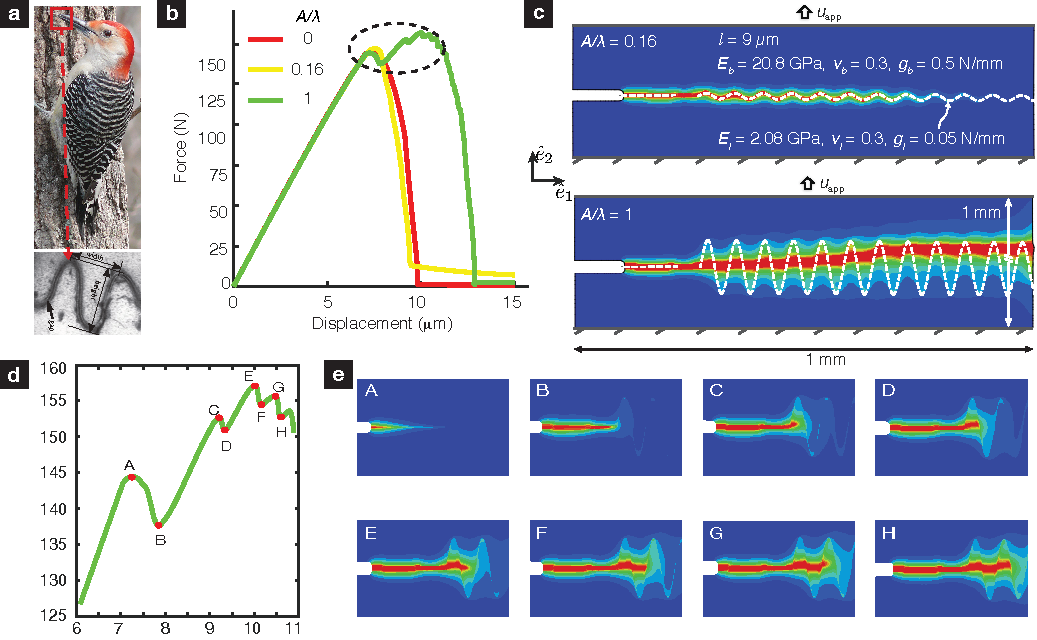
\includegraphics[width=\textwidth]{../../Proposal/ProjectDescription/Figures/WavyInterface//SinusoidalInterfaceFigCrackPropagation_V7.pdf}
	\centering	
	\caption{ (a) Wavy interfaces between keratin scales in the beak of the red bellied woodpecker (photo from [REF], micrograph reprinted from [REF]). (b) Load--displacement curves for different aspect ratios $A/\lambda$ of the interface shown in (c). (c) The crack propagates along a wavy interface for $A/\lambda = 0.16$. In comparison, the crack repeatedly ventures out of the interface into the bulk and then back into the interface through a series of instabilities, respectively, for $A/\lambda = 1$. The interface is shown as a dashed line. The interface is shown as a dashed line. (d) Zoom-in view of the load-displacement curve indicated by dashed circle in (b) showing the instabilities during the crack propagation. (e) Snapshots at instability points as indicated in (d).
	%Simulations are performed with regularization parameter $l = 0.009$ and wavelength $\lambda=0.0625\;\rm{mm}$. The bulk material has shear modulus $G=8\;\rm{GPa}$, bulk modulus $K=17.33\;\rm{GPa}$, and energy release rate $G_c=0.5\;\rm{N/mm}$, which are ten times of those of the interface.
	}
	\label{fig:VRF-WI} 
\end{figure}



The above examples reveal two interface toughening mechanisms including the instabilities induced by the unstable crack propagation through bulk material and the nucleations of secondary crack ahead of the primary crack, which cannot be captured by the CZM and XFEM simulations. The preliminary results suggest that the RVFM is a powerful approach through which we can investigate the intrinsic mechanisms of interface toughening for brittle fracture. It can also provide insights to analytically study the continuum model of interface toughening of brittle fracture.


\subsection{Current work--Short version}
 One of the primary differences between the wavy surface adhesion and wavy interface fracture problems is that in the case of fracture, a crack is not required to travel along the interface as it is in the adhesion problem. 
 %
 Rather, in the fracture problem, the crack can either travel along the interface or propagate through the bulk (see Figure~\ref{fig:VRF-WI}~(c)). The RVFT tool is ideally suited to handle this additional level of complexity.



% As illustration examples, we consider two elastic solids bonded by adhesive joint, as shown in Figure~\ref{fig:VRF-WI} (b)--(e). 
% %
% The upper and lower solids have the same material properties, i.e., shear modulus 8 GPa, bulk modulus 17.33 GPa, and energy release rate 0.5 N/mm. 
% %
% The adhesive joint has shear modulus 0.8 GPa, bulk modulus 1.733 GPa, and energy release rate 0.05 N/mm. 
% %
% The adhesive joint forms an interface with thickness 0.004 mm. 
% %
% Both straight and sinusoidal interfaces are investigated to study the effect of interface geometry on the fracture toughness. 
% %
% For the sinusoidal interface, the amplitude is $A$ and the wavelength is $\lambda$, and an straight interface with length $0.16\;\rm{mm}$ is introduced ahead of it. 
% %
% Moreover, a notch with length $0.11\;\rm{mm}$ is generated in the front of the interface. The bottom of the solid is fixed and a displacement $\Delta u$ is applied in $\hat{e}_2$ direction at the top (i.e., displacement controlled).


% We performed three different simulations, i.e., straight interface ($A = 0$) and wavy interfaces ($A = 0.01,0.0625\;\rm{mm}$) with wavelength $\lambda=0.0625\;\rm{mm}$ for regularization parameter $l = 0.009$. 
% %
% Figure~\ref{fig:VRF-WI} (c) show the crack propagation path for wavy interface with $A = 0.01\;\rm{mm}$ and $A=0.0625 \;\rm{mm}$, respectively. 
% %
% For small amplitude interface, the crack propagates along the interface. 
% %
% While for large amplitude, the crack path is no longer within the interface, instead it propagates through the bulk material. 
% %
% The load-displacement curves for $A=0$ and $A=0.01\;\rm{mm}$ are very similar (Figure~\ref{fig:VRF-WI} (b)). 
% %
% There is essentially no fracture toughness enhancement. 
% %
% However when $A$ increases from 0.01 to 0.0625 mm, the peak load is increased by $6.8\%$ from 147 to 157.2 N and the fracture toughness is increased by $55.3\%$ from 0.85 to 1.32 mJ. 
% %
% A series of instabilities are identified during the crack propagation in the large amplitude interface case, as shown in Figure~\ref{fig:VRF-WI} (e). 
% %
% The first unstable load drop corresponds to the unstable crack grows in the leading straight interface ($A \to B$). 
% %
% Once the crack hits the wavy interface the load builds up again until point $C$, after which the second unstable drop occurs. 
% %
% The second instability results from the unstable crack propagation through the bulk material ($C \to D$). 
% %
% Then the load increases again after the crack tip hit the wavy interface again. 
% %
% Several similar instabilities are observed subsequently, such as $E \to F$ and $G \to H$. 
% %
% The instabilities increase the maximum load that the specimen can sustain and make the failure process ductile, hence enhance the toughness.




As preliminary research, we implemented non-linear finite element techniques~\cite{belytschko2013nonlinear} to
numerically solve the RVFT Eqns.~\eqref{eq:GE} using the algorithms presented in \cite{borden2012phase}. 
%
The results of these calculations are shown in Figures~\ref{fig:VRF-PR}--\ref{fig:VRF-WI}. 
%
These results were generated for the special case of small deformations and $\Psi_0$ corresponding to the strain energy density of a homogeneous, isotropic, linear elastic material model.
%
We found that in many important cases the results of the RVFT match the predictions of linear elastic fracture mechanics (LEFM), see, e.g.,  Figure~\ref{fig:VRF-PR} (a).
%
It has also been shown that the crack path predicted by the RVFT matches the crack path seen in many experiments~\cite{miehe2010phase,borden2012phase,dally2015phase}. 
%
We were also able to reproduce these results, e.g., see Figure~\ref{fig:VRF-PR} (b).


The PI has performed a preliminary study of crack propagation in materials with wavy interfaces using the RVFT tool (see Figure~\ref{fig:VRF-WI}~(b)--(c)). 
%
In these simulations we allowed $g_c$ to vary spatially, so that in most of the solid it had a high value, $g_{b}$, and at a predefined wavy interface of finite thickness, it had a low value, $g_{I}$. 
%
In our preliminary simulations depending on the parameters $A/\lambda$ and $g_{I}/g_{b}$ the failure of the interface displayed very rich mechanics. 
%
Here, $A$ and $\lambda$ are the amplitude and the wavelength of the interface, respectively. 
%
For example, we found that at small $A/\lambda$ the crack always propagated along the interface (see Figure~\ref{fig:VRF-WI}~(c)). 
%
However, at larger $A/\lambda$ the crack repeatedly ventured out of the interface into the bulk and then back into the interface through a series of energy dissipating instabilities, see Figure~\ref{fig:VRF-WI}~(c). 
%
This lead to substantial toughening in the load-displacement response---i.e., area under the load-displacement curve (see Figure~\ref{fig:VRF-WI}~(b)).
%
The peak load is increased by 6.8\% and the fracture toughness is enhanced by 55.3\%. 
%
%
\begin{figure}[h]
	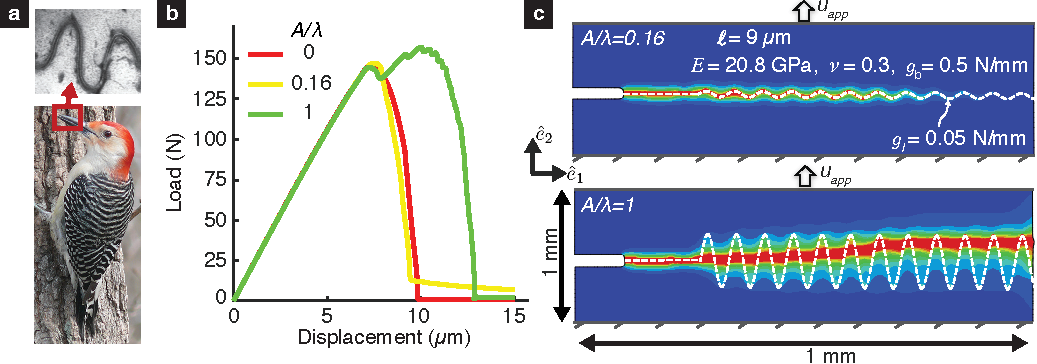
\includegraphics[width=\textwidth]{../../Proposal/ProjectDescription/Figures/WavyInterface//SinusoidalInterfaceFigCrackPropagation_V8.pdf}
	\centering	
	\caption{ (a) Wavy interfaces between keratin scales in the beak of the red bellied woodpecker (photo from [REF], micrograph reprinted from [REF]). (b) Load--displacement curves for different aspect ratios $A/\lambda$ of the interface shown in (c). (c) The crack propagates along a wavy interface for $A/\lambda = 0.16$. In comparison, the crack repeatedly ventures out of the interface into the bulk and then back into the interface through a series of instabilities, respectively, for $A/\lambda = 1$. The interface is shown as a dashed line.
	}
	\label{fig:VRF-WI} 
\end{figure}



The above examples reveal two interface toughening mechanisms including the instabilities induced by the unstable crack propagation through bulk material and the nucleations of secondary crack ahead of the primary crack, which cannot be captured by the CZM and XFEM simulations. The preliminary results suggest that the RVFM is a powerful approach through which we can investigate the intrinsic mechanisms of interface toughening for brittle fracture. It can also provide insights to analytically study the continuum model of interface toughening of brittle fracture.
% \newpage
% \bibliographystyle{unsrt}
% \bibliography{Refs_InterfaceToughening}

\end{document}